% FUNDAMENTAÇÃO TEÓRICA--------------------------------------------------------

\chapter{FUNDAMENTAÇÃO TEÓRICA}
\label{chap:fundamentacao-teorica}

\section{Double-multiple streamtube model - DMST}
\label{sec:dmst}

Considerando a \autoref{fig:EsquemaVelocidade} que apresenta o comportamento das velocidades envolvidas em uma pá, a velocidade relativa ($u_r$) pode ser calculada pela \autoref{eq:Vrelativa}, o ângulo de trajetória ($\beta$) pela \autoref{eq:beta} e o ângulo de ataque ($\alpha$) pela \autoref{eq:alfa}, todos em função do ângulo azimute ($\theta$) da turbina.

\begin{figure}
	\centering
	\caption{Esquema do escoamento e forças na pá.}
	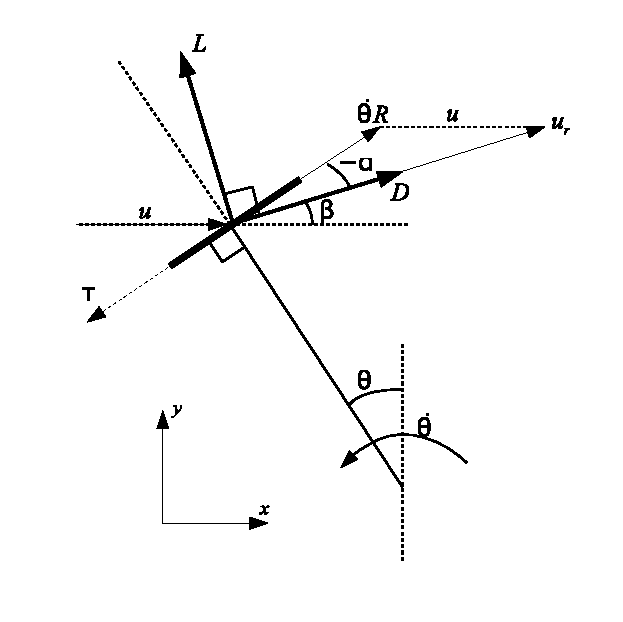
\includegraphics[width=0.7\textwidth]{figuras/EsquemaVelocidade.pdf}
	\fonte{ \citeonline{vallverdu2014}}
	\label{fig:EsquemaVelocidade}
\end{figure}

%Modelo de inclusão de equação. É só copiar, tomar como modelo e modificar.
\begin{equation}
{u_r} = \sqrt {{u^2} + {{(\dot \theta R)}^2} + 2u(\dot \theta R)\cos \theta }
\label{eq:Vrelativa}
\end{equation}

\begin{equation}
\beta  = \arctan \left( {\frac{{\dot \theta Rsen\theta }}{{u + \dot \theta R\cos \theta }}} \right)
\label{eq:beta}
\end{equation}

\begin{equation}
\alpha  = \left| {\frac{{\pi  + \beta  - \theta }}{{2\pi }}} \right| - \pi
\label{eq:alfa}
\end{equation}

Uma vez que o angulo de ataque é conhecido os coeficiente de sustentação ($C_L$) e arrasto ($C_D$) podem ser obtidos. Assim as forças de sustentação ($L$) e arrasto ($D$) podem ser calculadas conforme \autoref{eq:L} e \autoref{eq:D}, respectivamente. Sendo $\rho$ a massa específica do fluido, $c$ a corda, ....

\begin{equation}
L = \frac{1}{2}\rho cu_r^2{C_L}
\label{eq:L}
\end{equation}

\begin{equation}
D = \frac{1}{2}\rho cu_r^2{C_D}
\label{eq:D}
\end{equation}


\section{Modelagem dinâmica}
\label{sec:modelagemdinamica}
